\documentclass{beamer}
\usepackage[utf8]{inputenc}
\usepackage[french]{babel}
\usepackage{graphics}
\usepackage{multirow}
\usepackage{colortbl}
\usepackage{CJKutf8}

%\usepackage[screen,nopanel]{pdfscreen}
%\usepackage{url}

\usetheme{metropolis}

\title{Projet agile N4}
\author{
  %\includegraphics[width=3cm]{logo_azae.png}
  Thomas Clavier \\
  Julien Marchal \\
  Yann Secq 
}
  
\date{}

\logo{
  \raisebox{-0.5\height}{\includegraphics[width=1cm]{cc_by_sa} }
}


\begin{document}

\frame{\titlepage}

\begin{frame}{Suivre nos pieds}
  \Large Si vous n’apprenez rien ou que vous ne contribuez pas, passez à autre chose !
\end{frame}

\begin{frame}{C'est quoi ?}
 
  {\Large \alert{Être agile} et pas faire de l'Agile.}

  \vspace{6mm}
  C'est avant tout un état d'esprit partagé par l'ensemble des participants à un projet.
\end{frame}

\begin{frame}{Être agile}
  "Les firmes qui survivent dans le long terme ne sont pas celles qui sont les plus fortes ou les plus intelligentes, mais celles qui s'adaptent le mieux aux changements d'environnement"

  \flushright{Hiroshi Okuda, Toyota}

\end{frame}

\begin{frame}{Le manifeste agile}
  \large
  \alert{Individuals and interactions} over processes and tools\newline
  \alert{Working software} over comprehensive documentation\newline
  \alert{Customer collaboration} over contract negotiation\newline
  \alert{Responding to change} over following a plan
\end{frame}

\begin{frame}{Valeurs et principes}
  \Large Des cycles courts, un produit en production à chaque fin de cycle et des producteurs de valeurs qui s'améliorent continuellement.
\end{frame}

\begin{frame}{Le radiateur d'information}
  \begin{itemize}
    \item Donner les moyens aux acteurs d'être autonome
    \item Faire rayonner l'information
    
    \begin{itemize}
      \item Vision du projet, Proposition de valeur unique
      \item Date de livraison, avancement, etc.
      \item Planning des congés
      \item Actions d'améliorations
      \item Backlog
      \item Problèmes
      \item Etc.
    \end{itemize}
  \end{itemize}
\end{frame}

\begin{frame}{Exemple de radiateur}
  \center
  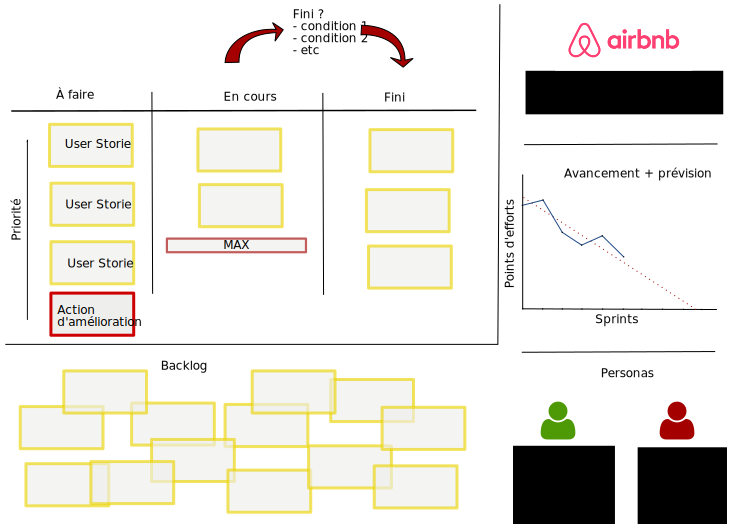
\includegraphics[width=10cm]{includes/radiateur}
\end{frame}

\begin{frame}{Kaizen 
    {\begin{CJK*}{UTF8}{mj} 改善 \end{CJK*}}
  }
  \center
  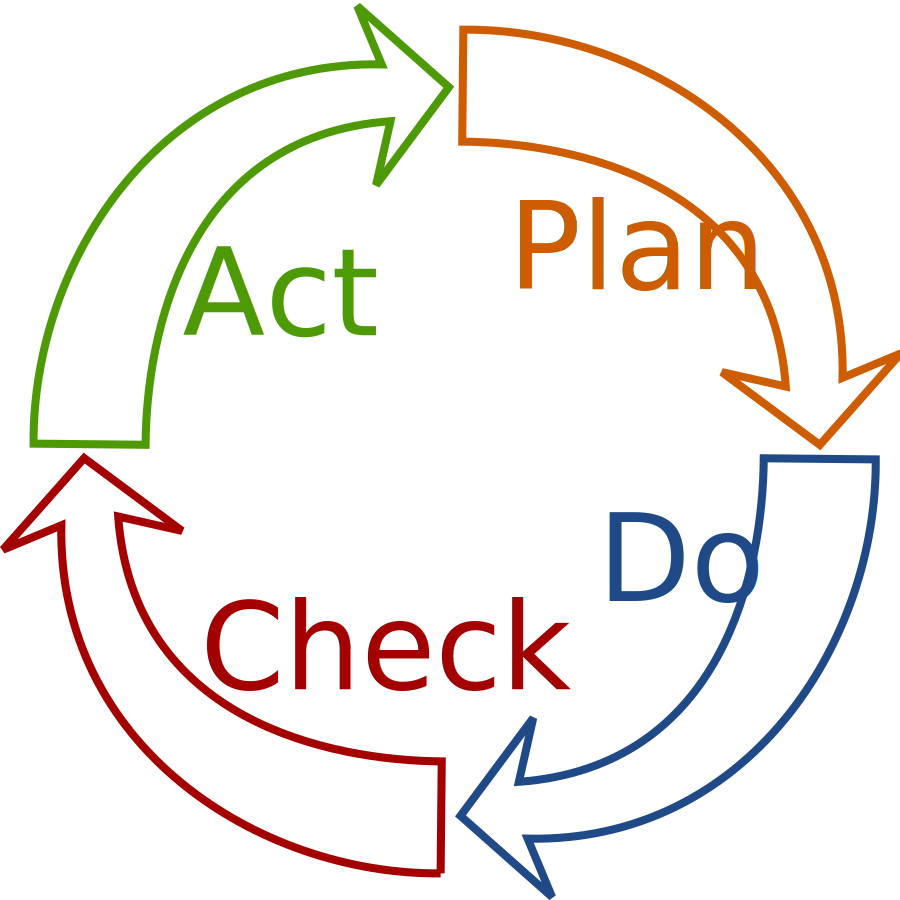
\includegraphics[width=6cm]{includes/pdca}
\end{frame}

\begin{frame}{Kaizen 
    {\begin{CJK*}{UTF8}{mj} 改善 \end{CJK*}}
  }
  
  \begin{itemize}
    \item \alert{Plan} : Identifier une action d'amélioration et un élément observable qui pourra permettre de déterminer si l'action à porté ses fruits ou pas.
    \item \alert{Do} : faire l'action sur un temps donné, une itération par exemple.
    \item \alert{Check} : Prendre le temps de mesurer si l'action a apporter le changement souhaité
    \item \alert{Act} : Décider, l'action est peut-être à répéter, une autre action peu en découler, etc.
  \end{itemize}

\end{frame}

\newcolumntype{g}{>{\columncolor[gray]{0.8}}c}

\begin{frame}{Planning de la semaine}{}
  {
    \center
    \begin{tabular}{l | g | g | g || c | c | }
      & \textbf{23/03} & \textbf{24/03} & \textbf{25/03} & \textbf{29/03} & \textbf{30/03} \\
      \hline
      08h00 - 10h00 & Sprint B & Sprint & Sprint & Sprint & Sprint \\
      \hline
      10h00 - 12h00 & Sprint 0 & Sprint & Sprint & Sprint & Sprint \\
      \hline
      \hline
      13h30 - 15h30 & Sprint & Sprint &                              & Sprint & \multirow{2}{*}{Salon} \\
      \cline{1-3} \cline{5-5}        
      15h30 - 17h30 & Sprint & Sprint & \multirow{-2}{*}{Soutenance} & Sprint & \\
      \hline
    \end{tabular}
  }

  \textcolor{gray}{\rule{2ex}{1.5ex}} : Info + GEA
\end{frame}

\begin{frame}{Un Sprints}
  \begin{itemize}
    \item 1,5h de production
    \item 30 minutes pour améliorer la capacité de production
    \begin{itemize}
      \item Démo
      \item Rétrospective
      \item Action d'amélioration
      \item Pause
    \end{itemize}
  \end{itemize}
\end{frame}

\begin{frame}{Détail des Sprints B et 0}
  Une matinée, 4 Objectifs : 
  \begin{itemize}
    \item Partager la vision du produit
    \item Découper et estimer le backlog
    \item Construire la proposition de valeur unique :
    \begin{itemize}
      \item Cible
      \item Problème
      \item Solution
    \end{itemize}
    \item Initier la pile technique et montrer que l'on est capable de livrer de la valeur.
  \end{itemize}
\end{frame}

\begin{frame}{Soutenance}
  Imaginez que vous devez levez des fonds, il faut convaincre sur la viabilité économique et technique de votre projet en 5 diapos, c'est l'elevator pitch.
  \begin{itemize}
    \item Identité visuelle et proposition de valeur unique
    \item Présentation de l'équipe
    \item Détail de la raison (why) : pourquoi cette idée innovante ?
    \item La solution face à la concurance 
    \item Le marché, le modèle économique
    \item Démo
  \end{itemize}

  Maximum 5 min sans les questions.
\end{frame}

\begin{frame}{Salon}
  Imaginez que vous devez vendre votre produit aux visiteurs du salon
  \begin{itemize}
    \item Un stand pour montrer les avantages de votre produit
    \item Présentation de l'équipe
    \item 
    \item La solution face à la concurance 
    \item Le marché, le modèle économique
    \item Démo
  \end{itemize}

  Maximum 5 min sans les questions.
\end{frame}
\end{document}

